\recipe{Tzatziki}
\label{rec:tzatziki}
\worktime{10 minutes}
\totaltime{10 minutes}
\makes{Makes enough for three as a side}

\begin{ingredients}
    \item Yoghurt, \SI{1}{\cup}
    \item Cucumber, 1 cubed
    \item Lemon juice, \SI{1}{\tablespoon}
    \item Olive oil, \SI{1}{\tablespoon}
    \item Salt, \SI{0.25}{\teaspoon}
    \item Garlic, 1 clove grated
    \item Dill, \SI{1}{\tablespoon}
    \item Mint, \SI{1}{\tablespoon}
\end{ingredients}

\begin{method}
Mix together and serve.
\end{method}


\begin{figure}[h]
  	\centering
  	
  	\begin{tikzpicture}
  		% Save the image in a box to get its dimensions
  		\sbox0{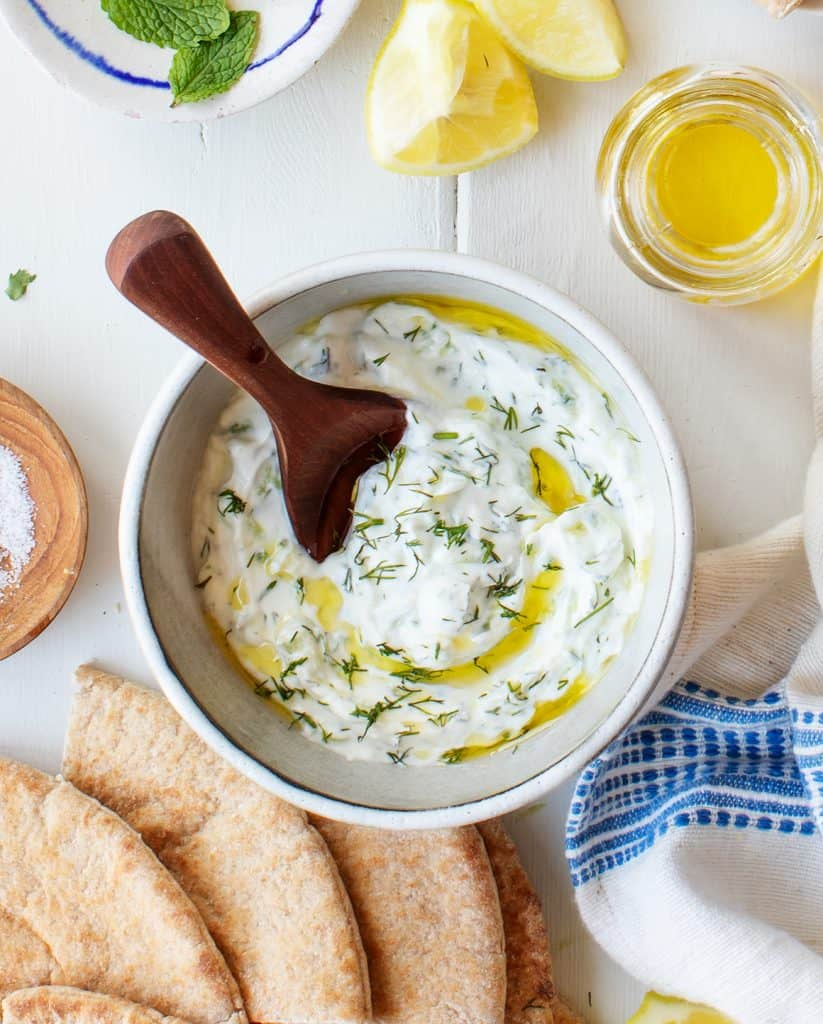
\includegraphics[height=7cm]{images/tzatziki-recipe-1-823x1024.jpg}}%
  
  		% Draw a clipping rectangle with rounded corners
  		\path[clip, rounded corners=0.5cm] (0,0) rectangle (\wd0,\ht0);
  
  		% Place the image inside the clipped area
  		\node[inner sep=0pt, outer sep=0pt, anchor=south west] at (0,0) {\usebox0};
	\end{tikzpicture}

  \caption*{}
\end{figure}